% ------------------------------------------------------------------------
% bjourdoc.tex for birkjour.cls*******************************************
% ------------------------------------------------------------------------
%%%%%%%%%%%%%%%%%%%%%%%%%%%%%%%%%%%%%%%%%%%%%%%%%%%%%%%%%%%%%%%%%%%%%%%%%%

\documentclass{birkjour}
%
%
% THEOREM Environments (Examples)-----------------------------------------
%
 \newtheorem{thm}{Theorem}[section]
% \newtheorem{cor}[thm]{Corollary}
% \newtheorem{lem}[thm]{Lemma}
% \newtheorem{prop}[thm]{Proposition}
% \theoremstyle{definition}
 \newtheorem{defn}[thm]{Definition}
% \theoremstyle{remark}
% \newtheorem{rem}[thm]{Remark}
% \newtheorem*{ex}{Example}
 \numberwithin{equation}{section}

\usepackage[noadjust]{cite}
\usepackage{amsfonts}
\usepackage{listings}
\usepackage{algorithm}
\usepackage{algorithmic}
\usepackage{booktabs}
\usepackage{float}
\usepackage{caption}

\begin{document}

%-------------------------------------------------------------------------
% editorial commands: to be inserted by the editorial office
%
%\firstpage{1} \volume{228} \Copyrightyear{2004} \DOI{003-0001}
%
%
%\seriesextra{Just an add-on}
%\seriesextraline{This is the Concrete Title of this Book\br H.E. R and S.T.C. W, Eds.}
%
% for journals:
%
%\firstpage{1}
%\issuenumber{1}
%\Volumeandyear{1 (2004)}
%\Copyrightyear{2004}
%\DOI{003-xxxx-y}
%\Signet
%\commby{inhouse}
%\submitted{March 14, 2003}
%\received{March 16, 2000}
%\revised{June 1, 2000}
%\accepted{July 22, 2000}
%
%
%
%---------------------------------------------------------------------------
%Insert here the title, affiliations and abstract:
%


\title[A High-Performance Orientation Estimator in Geometric Algebra]
 {A High-Performance Orientation Estimator in Geometric Algebra}

%----------Author 1
\author[Mauricio Cele Lopez Belon]{Mauricio Cele Lopez Belon}
\address{Buenos Aires, Argentina}
\email{mclopez@outlook.com}

%\thanks{This work was completed with the support of our \TeX-pert.}
%----------Author 2
%\author[Jin Wu]{Jin Wu}
%\address{University of Electronic Science and Technology of China, Chengdu, China}
%\email{jin\_wu\_uestc@hotmail.com}

%----------classification, keywords, date
\subjclass{Parallel algorithms 68W10; Clifford algebras, spinors 15A66}

\keywords{Geometric Algebra, Rotation Estimation, Wahba Problem}

\date{October 31, 2016}
%----------additions
%\dedicatory{To my wife}
%%% ----------------------------------------------------------------------

\begin{abstract}

Modern microprocessors supporting Advanced Vector Extensions (AVX) can double the speed of calculations on floating point data. By leveraging the available $4\times 4$ matrix multiplication routines using AVX registers, we developed a high-performance estimator of the best rotation aligning two sets of corresponding vectors (also known as Wahba's problem). On modern micro-processors, the proposed method outperform the fastest methods reported in literature and on old microprocessors it is still among the fastest methods, moreover it is robust to noise, accurate and simpler than most other methods. Our solution is based on Geometric Algebra representation of rotations which is isomorphic to Hamilton's quaternions.

\end{abstract}

%%% ----------------------------------------------------------------------
\maketitle
%%% ----------------------------------------------------------------------
%\tableofcontents
\section{Introduction}

\indent Wahba's problem has been studied for over half a century since 1965 \cite{Wahba1965}. The problem looks for the optimal rotation between two sets of corresponding vectors. Many effective algorithms have been developed to solve the problem \cite{Arun1987, Horn1987, Mortari1996, Shuster1981, Wu2017, Yang2015} using quaternions, the Singular Value Decomposition (SVD) and recently geometric algebra representation \cite{Perwass2009, Dorst2011}. Applications of Wahba's solutions are diverse from aerospace engineering computation of spacecraft attitude \cite{Wu2017} to mesh deformation in computer graphics \cite{Sorkine2007, Sin2013} for accurate motion construction and restoration \cite{Nieto2012, Perwass2009}.

In engineering fields requiring high performance vector alignment our method can lowered down the time in more than 50\% by leveraging the Advanced Vector Extensions (AVX) support available in modern microprocessors. In this work we propose a fast, robust to noise, simple and accurate method for solving the Wahba's problem. It is based on minimizing a convex least squares error formulated in geometric algebra $\mathbb{G}_3$. The proposed method allow us to exploit the available AVX instructions to accelerate the $4\times 4$ matrix multiplication of symmetric matrix. Obtaining a performance boost not present in other numerical algorithms when execute on modern hardware.

Few work has been done on studying this problem using geometric algebra. Geometric algebra rotors are closely related to quaternions (quaternion algebra can be regarded as a geometric algebra defined on a set of imaginary basis vectors) we find geometric algebra to be a more natural choice for studying this problem since it is defined over a Euclidean vector space $\mathbb R^3$, where original data is defined. We derive our algorithm from Wahba's problem defined on bivectos instead of vectors for the sake of mathematical simplicity. Due to mathematical duality of vector and bivectors in $\mathbb{G}_3$ our formulation is also valid for vectors. The implementation of our algorithm does not require access to any geometric algebra library, we present an implementation based on standard matrix and quaternion library. 

\indent This paper is arranged as follows: Section II introduces the geometric algebra $\mathbb{G}_3$, Section III includes the presentation of our fast rotor estimation algorithm. Section IV demonstrates the experimental results.

\section{Geometric Algebra $\mathbb{G}_3$}

A geometric algebra $\mathbb{G}_3$ is constructed over a real vector space $\mathbb R^3$, with basis vectors $\{e_1, e_2, e_3\}$. The associative geometric product is defined so that the square of any vector is a scalar $a a = a^2 \in \mathbb{R}$. From the vector space $\mathbb R^3$, the geometric product generates the geometric algebra $\mathbb{G}_3$ with elements $\{ X, R, A...\}$ called multivectors.

For a pair of vectors, a symmetric inner product $a \cdot b = b \cdot a$ and antisymmetric outer product $a \wedge b = -b \wedge a$ can be defined implicitly by the geometric product $a b = a \cdot b + a \wedge b$ and $b a = b \cdot a + b \wedge a$. It is easy to prove that $a \cdot b = \frac{1}{2}(a b + b a)$ is scalar, while the quantity $a \wedge b = \frac{1}{2}(a b - b a)$, called a bivector or $2$-vector, is a new algebraic entity that can be visualized as the two-dimensional analogue of a direction, that is, a planar direction. Similar to vectors, bivectors can be decomposed in a bivector basis $\{ e_{12}, e_{13}, e_{23} \}$ where $e_{ij} = e_i \wedge e_j$.

The outer product of three vectors $a \wedge b \wedge c$ generates a $3$-vector also known as the pseudoscalar, because the trivector basis consist of single element $e_{123} = e_1 \wedge e_2 \wedge e_3$. Similarly, the scalars are regarded as $0$-vectors whose basis is the number $1$. It follows that the outer product of $k$-vectors is the completely antisymmetric part of their geometric product: $a_1 \wedge a_2 \wedge ... \wedge a_k = \langle a_1 a_2 ... a_k \rangle_k$ where the angle bracket means $k$-vector part, and $k$ is its grade. The term grade is used to refer to the number of vectors in any exterior product. This product vanishes if and only if the vectors are linearly dependent. Consequently, the maximal grade for nonzero $k$-vectors is $3$. It follows that every multivector $X$ can be expanded into its $k$-vector parts and the entire algebra can be decomposed into $k$-vector subspaces:
\begin{equation*}
\mathbb G_3 = \sum_{k=0}^n{\mathbb{G}^k_3} = \{ X = \sum_{k=0}^n { \langle X \rangle_k } \}
\end{equation*}
This is called a \emph{grading} of the algebra. 

Reversing the order of multiplication is called reversion, as expressed by $(a_1 a_2 ... a_k)\tilde{} = a_k ... a_2 a_1$ and $(a_1 \wedge a_2 \wedge ... \wedge a_k)\tilde{} = a_k \wedge ... \wedge a_2 \wedge a_1$, and the reverse of an arbitrary multivector is defined by $\tilde{X} = \sum_{k=0}^n { \langle \tilde{X} \rangle_k }$.

Rotations are even grade multivectors known as rotors. We denote the subalgebra of rotors as $\mathbb{G}^{+}_3$. A rotor $R$ can be generated as the geometric product of an even number of vectors. A reflection of any $k$-vector $X$ in a plane with normal $n$ is expressed as the sandwitch product $(-1)^k n X n$. The most basic rotor $R$ is defined as the product of two unit vectors $a$ and $b$ with angle of $\frac{\theta}{2}$. The rotation plane is the bivector $B = \frac{a \wedge b}{\| a \wedge b \|}$.
\begin{equation*}
a b = a \cdot b + a \wedge b = \cos\left( \frac{\theta}{2} \right) + B \sin\left( \frac{\theta}{2} \right).
\end{equation*}
Rotors act on all $k$-vectors using the sandwitch product $X' = R X \tilde R$, where $\tilde R$ is the reverse of $R$ and can be obtained by reversing the order of all the products of vectors.

\section{Geometric Algebra Rotor Estimation}

Given two sets of $n$ corresponding bivectors $P = \{p_j\}_{j=1}^n$ and $Q = \{q_j\}_{j=1}^n$, we attempt to minimize the following error function:
\begin{eqnarray*}
E(R) = \min_{R \in \mathbb{G}^{+}_3 } \sum_j { c_{j} \|q_j - R p_i \tilde R\|^2 }\\
s.t. \ R \tilde R = 1
\end{eqnarray*}
where $\{c_{j}\}_{j=1}^n$ are scalar weights such that $\sum_j^n{c_j} = 1$. In that form, the minimization is a non-linear least squares problem with a non-linear constraint in $R$. Notice that the error term $q_j - R p_i \tilde R$ is equivalent to $q_j R - R p_j$ by multiplying by $R$ on the right and using the fact that $R \tilde R = 1$. The equivalent problem is:
\begin{eqnarray*}
E(R) = \min_{R \in \mathbb{G}^{+}_3 } \sum_j { c_{j} \|R p_j - q_j R\|^2 }\\
s.t. \ R \tilde R = 1
\end{eqnarray*}
which is a linear least squares problem with a non-linear constraint in $R$.

We define the commutator product of two bivectors $p_j$ and $q_j$ as $p_j \times q_j = \frac{1}{2}(p_j q_j - q_j p _j)$. The commutator product of bivectors in $\mathbb{G}_3$  can be interpreted as a cross product of bivectors in the sense that the resulting bivector $B = p_j \times q_j$ is orthogonal to both $p_j$ and $q_j$.

For a pair of unit bivectors, $A$ and $B$, the rotor $R$ aligning them can be defined as $R = A \frac{(A + B)}{\|A + B\|}$. Define the unit bivector $C = \frac{A + B}{\|A + B\|}$ the rotor $R$ is also $R = A C = w + L$ where $w = A \cdot C = \cos(\theta/2)$ and $L = A \times C = \sin(\theta/2) \frac{A \times B}{\|A \times B\|}$.

The constraint $R p_j - q_j R = 0$ can be rewrite as $(w + L) p_j - q_j (w + L) = (w + L) \cdot (p_j - q_j) + L \times (p_j + q_j)$. Since the inner product $L \cdot (p_j - q_j) = 0$, the constraint can be seen as:

\begin{eqnarray*}
w (p_j - q_j) +  L \times (p_j + q_j)  = 0\\
L \times (p_j + q_j) = -w (p_j - q_j)\\
%\frac{\sin(\theta/2)}{\|p_j + q_j\|} (p_j + q_j) \times (p_j \times (p_j + q_j)) = \cos(\theta/2) (p_j - q_j) 
\end{eqnarray*}
The above constraint equation holds when the input data is not noisy, since all terms $(p_j - q_j) \cdot L$ cancels out. However in a realistic case the input data would have some level of noise so it is better to keep the term $(p_j - q_j) \cdot L$ in the equation and let the optimization find its minimum possible value:

\begin{eqnarray*}
(p_j - q_j) \cdot (w + L) + L \times (p_j + q_j) = 0\\
\end{eqnarray*}

In matrix language we can define the following matrix system $M_j R = 0$:
%\begin{eqnarray*}
%\left[\begin{array}{c|c}
%0             & p_j - q_j \\
%\hline
%-(p_j - q_j) & \left[ p_j + q_j \right]^T_\times \\
%\end{array}\right]
%\left[\begin{array}{c} w \\ L \end{array}\right] = 
%\left[\begin{array}{c} 0 \\ 0  \end{array}\right]\\
%\end{eqnarray*}
\begin{eqnarray*}
\left[\begin{array}{cc}
0             & -d^T \\
d & \left[ s \right]^T_\times \\
\end{array}\right]
\left[\begin{array}{c} w \\ L \end{array}\right] = 
\left[\begin{array}{c} 0 \\ 0  \end{array}\right]\\
d = p_j - q_j \ \ s = p_j + q_j
\end{eqnarray*}
where $M_j$ is skew-symmetric $4\times 4$ real matrix, so that $M_j^T = -M_j$. The rotor $R$ is represented as $4 \times 1$ column vector with the real scalar $w$ and a vector $L \in \mathbb R^3$ holding the bivector components. The $3\times 3$ skew-symmetric matrix $\left[ p_j + q_j \right]_\times$ is representing the cross-product matrix as defined for vectors in $\mathbb R^3$.

%Let $\mathcal K : \mathbb{G}^{+}_3 \mapsto \mathbb{R}^4$ be a function that maps a rotor to a $4\times 1$ column matrix. 
%\begin{eqnarray*}
%\mathcal K(R) = \left[\begin{array}{c} \langle R \rangle_0 \\ \langle R \rangle_{12} \\ \langle R \rangle_{13} \\ \langle R \rangle_{23} \end{array}\right]
%\end{eqnarray*}

Let define the function $F^j$ representing the linear transformation:
\begin{eqnarray*}
%F^j = \mathcal K(\sqrt{c_j} (R p_j - q_j R))\\
F^j = \sqrt{c_j} M_j R\\
\end{eqnarray*}
%with $M_j$ is defined as the following skew-symmetric $4\times4$ real matrix:
%\begin{eqnarray*}
%M_j = 
%\left[\begin{array}{cccc}
%0                       & \langle D \rangle_{12} & \langle D \rangle_{13}  & \langle D \rangle_{23}\\
%-\langle D \rangle_{12} &         0              & -\langle S \rangle_{23} & \langle S \rangle_{13}\\
%-\langle D \rangle_{13} & \langle S \rangle_{23} &          0              & -\langle S \rangle_{12}\\
%-\langle D \rangle_{23} & -\langle S \rangle_{13}& \langle S \rangle_{12}  &          0             \\
%\end{array}\right]\\
%D = q_j - p_j \ \ S = p_j + q_j
%\end{eqnarray*}
%For simplicity of notation we denote the rotor $R \in \mathbb{G}^{+}_3$ and vector $\mathcal K(R) \in \mathbb R^4$ with letter $R$.
%Note that $M_j^T = -M_j$ as $M_j$ is representing the non-commutativity of the geometric product as well as the antisymmetry of bivectors.

Let $F$ be a column vector of $n$ stacked functions $F^j$
\begin{eqnarray*}
F = \left[\begin{array}{c}F^1 \\ \vdots \\ F^n\end{array}\right]
\end{eqnarray*}
 such that the energy $E(R)$ can be expressed as matrix product
\begin{eqnarray*}
E(R) = F^T F =
\left[\begin{array}{ccc}F^{1T} & \cdots & F^{nT}\end{array}\right]
\left[\begin{array}{c}F^1 \\ \vdots \\ F^n\end{array}\right]
\end{eqnarray*}

We can express $E(R)$ as the following quadratic form:
\begin{eqnarray*}
E(R) = \min_R R^T M R\\
s.t. \ R^T R = 1
\end{eqnarray*}
where $M = \sum_j^n { c_j M_j^T M_j}$. Note that since $M_j$ is skew-symmetric, the product $M_j^T M_j$ is symmetric and positive semi-definite.
Consequently the matrix $M$ is also symmetric positive semi-definite. It follows that all eigenvalues of $M$ are real and $\lambda_i \geq 0$.

\begin{eqnarray*}
M_j^T M_j = 
\left[\begin{array}{cc}
\| d \|^2 & (s \times d)^T \\
s \times d & d d^T - \left[ s \right]^2_\times \\
\end{array}\right]\\
d = p_j - q_j \ \ s = p_j + q_j
\end{eqnarray*}
%\begin{eqnarray*}
%M_j^T M_j = 
%\left[\begin{array}{c|c}
%\| p_j - q_j \|^2 & (p_j + q_j) \times (p_j - q_j) \\
%\hline
%(p_j + q_j) \times (p_j - q_j) & (p_j - q_j)(p_j - q_j)^T - \left[ p_j + q_j \right]^2_\times \\
%\end{array}\right]\\
%\end{eqnarray*}

Using the spectral theorem it is easy to show that the minimizer of $E(R)$ is the eigenvector of $M$ associated with the minimum eigenvalue.
Typically it can be obtained with great precision using SVD or QR factorization.
Nevertheless, in this work we seek for an efficient solution which allow us to take advantage of nowadays computing hardware.

The first row of $M_j$ is encoding the product $(p_j - q_j) \cdot L$ which is zero when the rotor $R$ aligns perfectly the input data. When that happen, $R$ is in the null space of $M_j$, the matrix $M_j^T M_j$ is singular as at least one eigenvalue is zero $\lambda_{\min} = 0$ (two eigenvalues will be zero for a single pair of corresponding bivectors). That implies that the energy $E(R)$ is non-convex, its shape is similar to a sinusoidal wave with infinitely many points at minimum energy value, each one at rotor $R_i = e^{-(\theta + i \pi) L}$ for $i \in \mathbb N$. That means that the solution is in general non-unique.


%Let us analyse the critical points of the energy $E(R)$. The minimum is attained when the gradient vanishes $\nabla E(R) = 0$. The gradient has the following form:
%\begin{eqnarray*}
%g = \nabla E(R)\\
%g = \nabla (F^T F)\\
%g = 2 J^T F
%\end{eqnarray*}
%where $J$ is the Jacobian matrix of $F$. Since the energy $E(R)$ is purely quadratic in $R$, the solution for $\nabla E(R) = 0$ can be found by solving a linear system of equations. An optimal rotor is in the null space of matrix $J^T F$. Naturally, a solution in the null space of $J^T F$ can be approximated using the Newton's method. Due to linearity of the equation $(J^T F) R = 0$ w.r.t. $R$ the optimal increment for $E(R)$ is given by the Newton formula $\Delta R = H^{-1} (J^T F) R$, provided that the inverse of Hessian matrix $H^{-1}$ exists. Noting that since $J$ does not depend on $R$, i.e. is constant, the Hessian matrix $H$ takes the simple form:
%\begin{eqnarray*}
%H = \frac{\partial(2 J^T F R)}{\partial R} \\
%H = 2 J^T \frac{\partial F R}{\partial R}\\
%H = 2 J^T J
%\end{eqnarray*}
%Where $H$ is independent of $R$. It seem that an optimal solution can be approximated by solving a series of linear systems.
%\begin{eqnarray*}
%R_{i+1} = R_i - H^{-1} (J^T F) R_i
%\end{eqnarray*}
%
%However, even when $H$ is non-singular, the Newton iteration introduced above is not possible. Note that $J^j = M_j$ since:
%\begin{eqnarray*}
%J^j = \frac{\partial(F^j R)}{\partial R}\\
%J^j = \frac{\partial(M_j R )}{\partial R}\\
%J^j = M_j
%\end{eqnarray*}
%replacing in Newton's formula we get
%\begin{eqnarray*}
%R_{i+1} = R_i - H^{-1} (J^T F) R_i\\
%R_{i+1} = R_i - (J^T J)^{-1} (J^T J) R_i
%\end{eqnarray*}
%which is a consequence of the non-convexity of $E(R)$.
%
%One simple solution is to use the Tikhonov regularization on $H$ to approximate a pseudo-inverse $(H + \epsilon I)^{-1}$. Tikhonov regularization makes $H$ symmetric positive definite matrix, making the energy $E(R)$ convex. An optimal solution can then be approximated by solving the following series of linear systems.
%\begin{eqnarray*}
%R_{i+1} = R_i - (H + \epsilon I)^{-1} H R_i
%\end{eqnarray*}
%until convergence is reached in the sense that $|R_i - R_{i+1}|_1 < \xi$ for a small $\xi$. Where we use $R_0 = [1 \ 0 \ 0 \ 0]^T$. This algorithm has a number of advantages. Since pseudo-inverse Hessian $(H + \epsilon I)^{-1}$ is constant, it can be precomputed. Also the Hessian matrix $H$ is constant, so it can be precomputed as well. Although the computation is relatively cheap and this approach is fast, the convergence is relatively slow. The choice of a small $\epsilon$ does accelerate convergence but at the expense of accuracy. However an algorithm with improved convergence and higher accuracy can be obtained by adding a new regularization term to $R(R)$.

\section{Fast Geometric Algebra Rotor Estimation}

%The non-convex energy $E(R)$ can be made convex by adding a new term to it. We introduce a new rotor $R_i$ within a new function $D(R, R_i) = \sqrt{\epsilon} (R - R_i)$.
%The new term can be expressed as matrix product:
%\begin{eqnarray*}
%D^T D = \epsilon \|R - R_i\|^2
%\end{eqnarray*}
%with Jacobian 
%\begin{eqnarray*}
%J_D = \frac{\partial D}{\partial R} = \sqrt{\epsilon} I
%\end{eqnarray*}
%where $I$ is the $4\times4$ identity matrix. The convex energy now looks like this:
%\begin{eqnarray*}
%E_2(R, R_i) = F^T F + D^T D\\
%E_2(R, R_i) = \sum_j { c_{j} \|R p_j - q_j R\|^2 } + \epsilon \|R - R_i\|^2
%\end{eqnarray*}
%Where $0 < \epsilon < 1$ is constant but small. The regularization term $D^T D = \epsilon \|R - R_i\|^2$ helps on finding a solution \emph{shifted} by a small amount towards the direction $\delta D = \epsilon (R - R_i)$, so one can interpret the rotor $R_i$ as a target of displacement. Also note that using $R^T R = 1$ and $R_i^T R_i = 1$ we get $D^T D = \epsilon (1 - R^T R_i)$ which can be seen as a soft normalization constraint.
%
%Note that the Hessian matrix of $E^j = R^T M_j^T M_j R$ is $H^j = 2 M_j^T M_j$. The Newton's update is defined as $\Delta R = H^{-1} \nabla E(R)$. The gradient and Hessian have the following form:
%\begin{eqnarray*}
%\nabla E(R) = \nabla(F^T F + D^T D)\\
%\nabla E(R) = \frac{\partial (F^T F)}{\partial R} + \frac{\partial (D^T D)}{\partial R}\\
%\nabla E(R) = 2 (H R + \epsilon D)\\
%\nabla E(R) = 2 ((H + \epsilon I) R - \epsilon R_i)
%\end{eqnarray*}
%where $H$ is defined as $H = \sum_j {M_j^T M_j}$.
%\begin{eqnarray*}
%\frac{\partial \nabla E(R)}{\partial R} = 2 \frac{\partial(H R + \epsilon D)}{\partial R} \\
%\frac{\partial \nabla E(R)}{\partial R} = 2 \frac{\partial(H R)}{\partial R} + 2 \epsilon \frac{\partial(D)}{\partial R}\\
%\frac{\partial \nabla E(R)}{\partial R} = 2 (H + \epsilon I)\\
%\end{eqnarray*}
%The first order term $\nabla E(R)$ and the second order term $\frac{\partial \nabla E(R)}{\partial R}$ are strikingly similar, so the Newton update will simplify them along with the initial guess $R_0$. Replacing the above definitions in Newton's formula we get:
%\begin{eqnarray*}
%R_{i+1} = R_0 - (H + \epsilon I)^{-1} ((H + \epsilon I) R_0 - \epsilon R_i)\\
%R_{i+1} = \epsilon (H + \epsilon I)^{-1} R_i
%\end{eqnarray*}

The most time consuming task of the estimation is to compute the eigenvector of $M$ associated with the minimum eigenvalue. Sound numerical algorithms for computing eigenvectors of a real symmetric matrix are SVD, QR factorization and Jacobi iteration among others. These algorithms find all eigenvectors of a matrix. Since we are interested in finding an eigenvector with least eigenvalue, our best choice is to use the Inverse Power Method. Which have the following form:

\begin{eqnarray*}
R_{i+1} = \epsilon (M + \epsilon I)^{-1} R_i
\end{eqnarray*}

Where $\epsilon$ is a small real value $0 < \epsilon < 1$. The use of Tikhonov regularization makes $M$ symmetric positive-definite matrix, making the energy $E(R)$ convex. Note that the Hessian matrix of $E^j = R^T M_j^T M_j R$ is $H^j = 2 M_j^T M_j$, so the Hessian matrix $H = \sum_j {M_j^T M_j}$ of $E(R)$ is equal to the matrix $M$. The Tikhonov regularization makes the Hessian matrix positive-definite.

The Newton update formula shade some light on the shape of the energy near the rotor $R_i$. The Newton's update formula is defined as:
\begin{eqnarray*}
R_{i+1} = R_i - (H + \epsilon I)^{-1} (J^T F) R_i
\end{eqnarray*}
where $J$ is the Jacobian matrix of $E(R)$ and the gradient is $\nabla E(R) = (J^T F) R$. Notice that the Jacobian matrix $J^j$ of $F^j$ is $J^j = M_j$, so $J^T F = \sum_j {M_j^T M_j}$. The Newton's update depends only on the Hessian, since it is shaping the curvature of the $3$-sphere manifold.
\begin{eqnarray*}
R_{i+1} = R_i - (H + \epsilon I)^{-1} H R_i
\end{eqnarray*}
The Newton's iteration is just aligning $R_{i+1}$ towards the dominant eigenvector of $(H + \epsilon I)^{-1}$. Numerical experiments shown that the column of $(H + \epsilon I)^{-1}$ with higher L$1$-norm is already close to the dominant eigenvector, specially in the absence of noise.

Newton's method convergence is \emph{quadratic}. However, it has been established that convergence of power iteration is linear or \emph{geometric}, depending on the ratio of the largest eigenvalue to the second eigenvalue $\lambda_2 / \lambda_{\max}$ i.e., the method converges slowly if there is an eigenvalue close in magnitude to the largest eigenvalue.

A well-known algorithm for finding dominant eigenvectors of matrices consists of repeatedly squaring a matrix, renormalizing the matrix after each squaring. See \cite{Wilkinson1988}. In \cite{Kostlan1991} it is showed that the convergence of the repeated squaring is \emph{quadratic} and for real symmetric $N \times N$ matrices the average number of iterations required is O($\ln N + \ln \|\ln \epsilon\|$). Moreover, the following upper bound is provided $\frac{1}{\ln 2} [ \ln( 3 \sqrt{2} ( N ( N - 1 ) / 2 + N ) ) + 1 + \ln( 2 \ln N + \|\ln \epsilon\|) ] + 1$. Thus for a symmetric $4 \times 4$ matrix, taking a small $\epsilon = 10^{-13}$ the average number of iterations is $6$ and upper bound is $12$. That can be exploited for creating deterministic algorithms.

Several mathematicians have proved bounds on eigenvalues in terms of the value of the matrix. A simple test in \cite{brauer1946}, is based on the L$1$-norm of the columns nd rows. Let $a_{ij}$ be the elements, $R_i = \sum_j |a_{ij}|$ be the L$1$-norm of the $i$th row and $C_j = \sum_i |a_{ij}|$ the L$1$-norm of the $j$th column. Let $\mathcal R$ be the largest $R_i$ and $\mathcal C$ the largest $C_j$. Then for all eigenvalues $|\lambda| \leq \min(\mathcal R, \mathcal C)$. Since our matrix is symmetric the upper bound is the same for rows and columns. Going back to the power method, we see that after a small number of repeated matrix squaring, the dominant eigenvector correspond to the $j$th column having the largest $C_j$ value.

The convergence of our method can be accelerated by squaring the matrix $(H + \epsilon I)^{-1}$ a given number of times before doing the power iteration. We show that in computers with vector instructions our method outperforms previous methods.


%WILKINSON, J. H. (1965), “The Algebraic Eigenvalue Problem,” Oxford Univ. Press, New York. 
%Eric Kostlan, Statistical Complexity of Dominant Eigenvector Calculation, Journal of Complexity, Academic Press, 1991
%Brauer, Alfred. Limits for the characteristic roots of a matrix. Duke Math. J. 13 (1946), no. 3, 387--395. doi:10.1215/S0012-7094-46-01333-6. https://projecteuclid.org/euclid.dmj/1077473736

%We will see how we can choose a good initial guess later on. The choice of epsilon is more subtle, since it affects the accuracy of result as well. In general, a small epsilon gives better convergence but low accuracy, on the other hand a big epsilon gives slower convergence but good accuracy. The best compromise is always an engineering decision.

% We still need to provide a first guess $R_0$ for our method. In theory any random unit quaternion would work. In all our tests we used $R_0 = [1 \ \epsilon \ \epsilon \ \epsilon]$.
% However, if the optimal rotor is at $\pm \pi$ from $R_0$, that choice might cause the optimization get stuck. For example, given two sets of corresponding vectors $P = \{p_1=e_1, p_2=e_2\}$ and $Q = \{q_1=-e_1, q_2=-e_2\}$ which are rotated by $\pi$ radians to each other, the Hessian is diagonal, and its pseudo-inverse $H_2^{-1}$ is \emph{almost} having the reciprocal values of its diagonal, assuming $R_i = R_0$, the gradient $g(R_0)$ coincide with the first column of $H$, and so the product $H_2^{-1} g(R_0) = [1 \ 0 \ 0 \ 0]^T$ so the resulting rotor $R_{i+1} = R_0 - H_2^{-1} g(R_0) = [0 \ 0 \ 0 \ 0]^T$. In practice, we have never experienced this problem, even with synthetic data, since the Tikhonov regularization introduces a sufficient perturbation on the pseudo-inverse to get a non-zero $R_{i+1}$ which, after normalization, is useful as a feedback direction.

% Given an estimated rotor $R_{i+1}$ a necessary condition for it to the optimal is that the recurrence $R_{i+1} = R_0 - H_2^{-1} g_2(R_0,R_i)$ converge to a rotor $R^*$ in the sense that $|R_i - R_{i+1}| < \xi$ for a small $\xi$. That is true because if $R_{i+1}$ is already optimal, the small displacement induced by the regularization term $\sqrt{\epsilon} D(R_0,R_i)$ should increase the least squares error $E_2$ and the linear system should compute the last $R_{i+1} = R^*$ as it has less error. So regularization term can be seen as a feedback for reaching a stable $R^*$. Since the regularization term is only affecting the gradient, the computation is very cheap. The gradient $g(R_0)$ can be precomputed as well as the matrix $H_2^{-1}$, and the iteration is reduced to compute a matrix vector multiplication.

%\section{Optimal Computation of Jacobians}
%
%The differential of $F^j$ defined as $J^j = \frac{\partial F^j}{\partial R}$ is a $4\times4$ matrix which four columns are the directional derivatives of $F^j = \sqrt{c_j} (R p_j - q_j R)$ w.r.t rotor components on the basis $\mathbb{G}^{+}_3$:
%\begin{eqnarray*}
%J^j = \left[\begin{array}{cccc}\frac{\partial F^j}{\partial w} & \frac{\partial F^j}{\partial e_{12}} & \frac{\partial F^j}{\partial e_{13}} & \frac{\partial F^j}{\partial e_{23}}\end{array}\right]
%\end{eqnarray*}
%\begin{eqnarray*}
%\frac{\partial F^j}{\partial w} = \sqrt{c_j} (p_j - q_j)\\
%\frac{\partial F^j}{\partial w} = \sqrt{c_j}
%\left[\begin{array}{c}(p_j - q_j) \cdot e_1 \\ (p_j - q_j) \cdot e_2 \\ (p_j - q_j) \cdot e_3 \\ 0\end{array}\right]
%\end{eqnarray*}
%\begin{eqnarray*}
%\frac{\partial F^j}{\partial e_{12}} = \sqrt{c_j} (-(p_j+q_j) \cdot e_{12} + (p_j-q_j) \wedge e_{12})\\
%\frac{\partial F^j}{\partial e_{12}} = \sqrt{c_j}
%\left[\begin{array}{c}(p_j + q_j) \cdot e_2 \\ -(p_j + q_j) \cdot e_1 \\ 0 \\ (p_j - q_j) \cdot e_3\end{array}\right]
%\end{eqnarray*}
%\begin{eqnarray*}
%\frac{\partial F^j}{\partial e_{13}} = \sqrt{c_j} (-(p_j  + q_j) \cdot e_{13} + (p_j - q_j) \wedge e_{13})\\
%\frac{\partial F^j}{\partial e_{13}} = \sqrt{c_j}
%\left[\begin{array}{c}(p_j  + q_j) \cdot e_3 \\ 0 \\ -(p_j  + q_j) \cdot e_1 \\ -(p_j - q_j) \cdot e_2\end{array}\right]
%\end{eqnarray*}
%\begin{eqnarray*}
%\frac{\partial F^j}{\partial e_{23}} = \sqrt{c_j} (-(p_j + q_j) \cdot e_{23} + (p_j - q_j) \wedge e_{23})\\
%\frac{\partial F^j}{\partial e_{23}} = \sqrt{c_j}
%\left[\begin{array}{c} 0 \\ (p_j  + q_j) \cdot e_3 \\ -(p_j  + q_j) \cdot e_2 \\ (p_j - q_j) \cdot e_1\end{array}\right]
%\end{eqnarray*}
%
%So the full expression of $J^j$ is:
%
%\begin{eqnarray*}
%J^j = \sqrt{c_j}
%\left[\begin{array}{cccc}
%(p_j - q_j) \cdot e_1 & (p_j + q_j) \cdot e_2  & (p_j  + q_j) \cdot e_3  & 0\\ 
%(p_j - q_j) \cdot e_2 & -(p_j + q_j) \cdot e_1 & 0                       & (p_j  + q_j) \cdot e_3\\
%(p_j - q_j) \cdot e_3 & 0                      & -(p_j  + q_j) \cdot e_1 & -(p_j  + q_j) \cdot e_2\\ 
%0                     & (p_j - q_j) \cdot e_3  & -(p_j - q_j) \cdot e_2  & (p_j - q_j) \cdot e_1
%\end{array}\right]
%\end{eqnarray*}
%
%The gradient of $E(R)$ amounts to $g = \sum_j{J^{jT} F^j}$ and the symmetric matrix $H^j = J^{jT} J^j$ has a simple form:
%
%\begin{eqnarray*}
%S_1 = (q_j + p_j) \cdot e_1 \ , \ S_2 = (q_j + p_j) \cdot e_2 \ , \ S_3 = (q_j + p_j) \cdot e_3\\
%D_1 = (p_j - q_j) \cdot e_1 \ , \ D_2 = (p_j - q_j) \cdot e_2 \ , \ D_3 = (p_j - q_j) \cdot e_3
%\end{eqnarray*}

\section{Optimal Computation of the Hessian}

The symmetric matrix $H^j = M_j^T M_j$ has a simple form:

\begin{eqnarray*}
S_1 = \langle q_j + p_j \rangle_{12} \ , \ S_2 = \langle q_j + p_j \rangle_{13} \ , \ S_3 = \langle q_j + p_j \rangle_{23}\\
D_1 = \langle p_j - q_j \rangle_{12} \ , \ D_2 = \langle p_j - q_j \rangle_{13} \ , \ D_3 = \langle p_j - q_j \rangle_{23}
\end{eqnarray*}

\begin{eqnarray*}
H^j = M_j^T M_j =\\
\left[\begin{array}{cccc}
D_1^2 + D_2^2 + D_3^2    & D_3 S_2 - D_2 S_3      & D_1 S_3 - D_3 S_1     & D_2 S_1 - D_1 S_2\\ 
D_3 S_2 - D_2 S_3        & D_1^2 + S_3^2 + S_2^2  & D_1 D_2 - S_2 S_1     & D_1 D_3 - S_3 S_1 \\
D_1 S_3 - D_3 S_1        & D_1 D_2 - S_2 S_1      & D_2^2 + S_3^2 + S_1^2 & D_2 D_3 - S_3 S_2\\ 
D_2 S_1 - D_1 S_2        & D_1 D_3 - S_3 S_1      & D_2 D_3 - S_3 S_2     & D_3^2 + S_2^2 + S_1^2
\end{array}\right]
\end{eqnarray*}

Since $H^j$ is symmetric only $10$ out of $16$ elements need to be actually computed. Notice that the trace of $H^j$ is $Tr(H^j) = 2 \|p_j - q_j\|^2 + 2 \|p_j + q_j\|^2$ and $Tr(H) = 2 \sum_j {(\|p_j - q_j\|^2 + \|p_j + q_j\|^2)}$.

\section{Algorithms}

Although our algorithm is based on the inverse power method, which is an iterative algorithm, it always performs a fixed number of matrix squaring operations. Since the upper bound of iterations has been established and numerical tests confirms that no more iterations are needed to achieve the required accuracy. Opposite to other iterative algorithms, we don't need a random guess for $R_0$. The best $R_i$ is always calculated by matrix squaring. %In a simulation, we also can take $R_i$ from the outside and perform only one iteration of the optimization to quickly yield a non-optimal rotor for the next simulation step. We call the later the \emph{incremental} algorithm. We have used both choices in our experiments, with excellent results in both cases. In the later case, our experiments indicates that our algorithm preserves the sense of successive rotations.

The proposed method is shown in Algorithm~\ref{alg:FastRotorEstimation}. 

\begin{algorithm}
\begin{algorithmic}[1]
\REQUIRE {$P = \{p_{j}\}_{j=1}^n, Q = \{q_{j}\}_{j=1}^n, C = \{c_{j}\}_{j=1}^n$}
\STATE{$H = 0_{4\times4}, \epsilon = 1\times10^{-13}$}
\FOR{$j = 1$ \TO $n$}
\STATE{$S_1 = (q_j + p_j) \cdot e_{21} \ , \ S_2 = (q_j + p_j) \cdot e_{31} \ , \ S_3 = (q_j + p_j) \cdot e_{32}$}
\STATE{$D_1 = (p_j - q_j) \cdot e_{21} \ , \ D_2 = (p_j - q_j) \cdot e_{31} \ , \ D_3 = (p_j - q_j) \cdot e_{32}$}
\STATE{$H = H + $\\
$c_j
\left[\begin{array}{cccc}
D_1^2 + D_2^2 + D_3^2    & D_3 S_2 - D_2 S_3      & D_1 S_3 - D_3 S_1     & D_2 S_1 - D_1 S_2\\ 
D_3 S_2 - D_2 S_3        & D_1^2 + S_3^2 + S_2^2  & D_1 D_2 - S_2 S_1     & D_1 D_3 - S_3 S_1 \\
D_1 S_3 - D_3 S_1        & D_1 D_2 - S_2 S_1      & D_2^2 + S_3^2 + S_1^2 & D_2 D_3 - S_3 S_2\\ 
D_2 S_1 - D_1 S_2        & D_1 D_3 - S_3 S_1      & D_2 D_3 - S_3 S_2     & D_3^2 + S_2^2 + S_1^2
\end{array}\right]$}
\ENDFOR
\STATE{$H_1^+ = (H + \epsilon I)^{-1}$}
\FOR{$i = 1$ \TO $12$}
\STATE{$H_i^2 = H_i^+ H_i^+$}
\STATE{$H_{i+1}^+ = \frac{1}{Tr(H_i^2)} H_i^2$}
\ENDFOR
\STATE{$\mathcal C_j = \max_j \sum_k^4 | H_{12}^+(k, j) |, j = 1, ..., 4 $}
\STATE{$ R = normalize( \mathcal C_j )$}
\RETURN { $R(0) + R(1) e_{12} + R(2) e_{13} + R(3) e_{23}$ }
\end{algorithmic}
\caption{Fast Rotor Estimation}\label{alg:FastRotorEstimation}
\end{algorithm}
The C++ code using the Eigen library can be found in Listing~\ref{lst:cppcode}.

%The \emph{incremental} algorithm is best suited if we know that the two sets of vectors are almost aligned. Let us suppose that we already have suboptimal rotor estimation $R_{prev}$, perhaps calculated for a previous simulation step, that almost align the two sets of vectors. We can use $R_{prev}$ to form a direction $\delta D = \epsilon (R - R_{prev})$ which we integrate in the regularization term. So the new rotor estimation is given by $R_{i+1} = R_0 - (H + \epsilon I)^{-1} (g + \epsilon (R_{prev} - R_0))$. This can be seen as moving the loop from inside the \emph{standalone} algorithm to the outside. When a simulation provides a temporal coherence between consecutive simulation steps, the incremental estimation of rotations is a good choice, since incremental algorithm only requires to solve a linear system for computing the next best rotor. Provided that the simulation converge to stable sets of corresponding vectors, then incremental rotor estimation will converge to $R^*$. The Algorithm~\ref{alg:FastRotorEstimation_incremental} shows the complete algorithm.
%
%\begin{algorithm}
%\begin{algorithmic}[1]
%\REQUIRE {$P = \{p_{j}\}_{j=1}^n, Q = \{q_{j}\}_{j=1}^n, C = \{c_{j}\}_{j=1}^n, R_{prev}$}
%\STATE{$R_0 = [1,0,0,0]^T, H = 0_{4\times4}$}
%\FOR{$j = 1$ \TO $n$}
%\STATE{$S_1 = (q_{j} + p_{j}) \cdot e_1 \ , \ S_2 = (q_{j} + p_{j}) \cdot e_2 \ , \ S_3 = (q_{j} + p_{j}) \cdot e_3$}
%\STATE{$D_1 = (p_{j} - q_{j}) \cdot e_1 \ , \ D_2 = (p_{j} - q_{j}) \cdot e_2 \ , \ D_3 = (p_{j} - q_{j}) \cdot e_3$}
%\STATE{$H = H + $\\
%$c_j
%\left[\begin{array}{cccc}
%D_1^2 + D_2^2 + D_3^2    & D_1 S_2 - D_2 S_1      & D_1 S_3 - D_3 S_1     & D_2 S_3 - D_3 S_2\\ 
%D_1 S_2 - D_2 S_1        & S_2^2 + S_1^2 + D_3^2  & S_2 S_3 - D_3 D_2     & D_3 D_1 - S_1 S_3 \\
%D_1 S_3 - D_3 S_1        & S_2 S_3 - D_3 D_2      & S_3^2 + S_1^2 + D_2^2 & S_1 S_2 - D_2 D_1\\ 
%D_2 S_3 - D_3 S_2        & D_3 D_1 - S_1 S_3      & S_1 S_2 - D_2 D_1     & S_3^2 + S_2^2 + D_1^2
%\end{array}\right]$}
%\ENDFOR
%\STATE{$g = -\left[\begin{array}{cccc} H(0,0) & H(1,0) & H(2,0) & H(3,0) \end{array}\right]^T$} 
%\STATE{$\Delta R = (H + \epsilon I)^{-1} (g + \epsilon (R_{prev} - R_0))$}
%\STATE{$R = normalize(R_0 + \Delta R)$}
%\RETURN {$R(0) + R(1) e_{12} + R(2) e_{13} + R(3) e_{23}$}
%\end{algorithmic}
%\caption{Incremental Fast Rotor Estimation}\label{alg:FastRotorEstimation_incremental}
%\end{algorithm}

\section{Comparisons}

We select several representative methods e.g. FLAE \cite{Wu2017}, SVD \cite{Horn1987} and QUEST \cite{Shuster1981} to implement the algorithm. The Eigen library is employed to implement the SVD and QUEST. Another version of QUEST using the Newton iteration is also added for comparison. The tests are ran on a MacBook Pro 13' 2017 computer with the CPU of Intel 3.1GHz 4-core i5. The Visual Studio 2019 C++ compiler is used in our experiments. %The results are listed below (Table \ref{tab:roll}, \ref{tab:pitch}, \ref{tab:yaw}):

% \begin{table} [H]
% \centering
% \begin{minipage}[b]{1.0\textwidth}
% \caption{Roll RMSE (deg)}  
%  \label{tab:roll}
% \resizebox{1.0\textwidth}{!}{ 
% \begin{tabular}{cccccc}
% \toprule
% {Case}&{Proposed}&{SVD Horn 1987}&{FLAE 2017}&{QUEST Eigen 1981}&{QUEST Newton 1981}\\
% \midrule
% {1}&{$4.9426 \times 10^{-04}$}&{$4.3068 \times 10^{-05}$}&{$4.3068 \times 10^{-05}$}&{$4.3068 \times 10^{-05}$}&{$4.3068 \times 10^{-05}$}\\
% {2}&{$3.3673 \times 10^{-04}$}&{$5.9781 \times 10^{-05}$}&{$5.9781 \times 10^{-05}$}&{$5.9781 \times 10^{-05}$}&{$5.9781 \times 10^{-05}$}\\
% {3}&{$2.4912 \times 10^{+00}$}&{$4.3420 \times 10^{-01}$}&{$4.3420 \times 10^{-01}$}&{$4.3420 \times 10^{-01}$}&{$4.3420 \times 10^{-01}$}\\
% {4}&{$3.4014 \times 10^{+00}$}&{$5.9978 \times 10^{-01}$}&{$5.9978 \times 10^{-01}$}&{$5.9978 \times 10^{-01}$}&{$5.9978 \times 10^{-01}$}\\
% {5}&{$3.9992 \times 10^{+00}$}&{$4.3545 \times 10^{-01}$}&{$2.1560 \times 10^{+01}$}&{$4.3545 \times 10^{-01}$}&{$4.3649 \times 10^{-01}$}\\
% {6}&{$4.9857 \times 10^{-02}$}&{$4.9792 \times 10^{-03}$}&{$4.9792 \times 10^{-03}$}&{$4.9792 \times 10^{-03}$}&{$4.9792 \times 10^{-03}$}\\
% {7}&{$8.7731 \times 10^{-02}$}&{$8.1146 \times 10^{-03}$}&{$8.1146 \times 10^{-03}$}&{$8.1146 \times 10^{-03}$}&{$8.1146 \times 10^{-03}$}\\
% {8}&{$3.4008 \times 10^{+02}$}&{$5.9402 \times 10^{+01}$}&{$5.9402 \times 10^{+01}$}&{$5.9402 \times 10^{+01}$}&{$5.9402 \times 10^{+01}$}\\
% {9}&{$5.3870 \times 10^{+02}$}&{$7.7637 \times 10^{+01}$}&{$7.7638 \times 10^{+01}$}&{$7.7637 \times 10^{+01}$}&{$7.7637 \times 10^{+01}$}\\
% {10}&{$1.3513 \times 10^{+01}$}&{$1.4641 \times 10^{+00}$}&{$1.5824 \times 10^{+00}$}&{$1.4641 \times 10^{+00}$}&{$1.4641 \times 10^{+00}$}\\
% {11}&{$1.9366 \times 10^{+01}$}&{$2.0427 \times 10^{+00}$}&{$2.9300 \times 10^{+00}$}&{$2.0427 \times 10^{+00}$}&{$2.0427 \times 10^{+00}$}\\
% {12}&{$1.2517 \times 10^{+01}$}&{$2.0712 \times 10^{+00}$}&{$1.7328 \times 10^{+01}$}&{$2.0712 \times 10^{+00}$}&{$3.3679 \times 10^{+01}$}\\
% \bottomrule
% \end{tabular}}
% \end{minipage}

% \begin{minipage}[b]{1.0\textwidth}
% \caption{Pitch RMSE (deg)}  
%  \label{tab:pitch}
% \resizebox{1.0\textwidth}{!}{ 
% \begin{tabular}{cccccc}
% \toprule
% {Case}&{Proposed}&{SVD Horn 1987}&{FLAE 2017}&{QUEST Eigen 1981}&{QUEST Newton 1981}\\
% \midrule
% {1}&{$4.0745 \times 10^{-04}$}&{$4.0500 \times 10^{-05}$}&{$4.0500 \times 10^{-05}$}&{$4.0500 \times 10^{-05}$}&{$4.0500 \times 10^{-05}$}\\
% {2}&{$4.1322 \times 10^{-04}$}&{$5.3106 \times 10^{-05}$}&{$5.3106 \times 10^{-05}$}&{$5.3106 \times 10^{-05}$}&{$5.3106 \times 10^{-05}$}\\
% {3}&{$4.0623 \times 10^{+00}$}&{$4.0205 \times 10^{-01}$}&{$4.0205 \times 10^{-01}$}&{$4.0205 \times 10^{-01}$}&{$4.0205 \times 10^{-01}$}\\
% {4}&{$6.0567 \times 10^{+00}$}&{$5.2600 \times 10^{-01}$}&{$5.2600 \times 10^{-01}$}&{$5.2600 \times 10^{-01}$}&{$5.2600 \times 10^{-01}$}\\
% {5}&{$2.4391 \times 10^{+00}$}&{$3.9376 \times 10^{-01}$}&{$1.1799 \times 10^{+01}$}&{$3.9376 \times 10^{-01}$}&{$3.9469 \times 10^{-01}$}\\
% {6}&{$3.6311 \times 10^{-04}$}&{$4.0168 \times 10^{-05}$}&{$4.0168 \times 10^{-05}$}&{$4.0168 \times 10^{-05}$}&{$4.0168 \times 10^{-05}$}\\
% {7}&{$6.2653 \times 10^{-04}$}&{$5.3300 \times 10^{-05}$}&{$5.3300 \times 10^{-05}$}&{$5.3300 \times 10^{-05}$}&{$5.3300 \times 10^{-05}$}\\
% {8}&{$4.3060 \times 10^{+00}$}&{$3.6817 \times 10^{-01}$}&{$3.6817 \times 10^{-01}$}&{$3.6817 \times 10^{-01}$}&{$3.6817 \times 10^{-01}$}\\
% {9}&{$5.9480 \times 10^{+00}$}&{$4.5583 \times 10^{-01}$}&{$4.5583 \times 10^{-01}$}&{$4.5583 \times 10^{-01}$}&{$4.5583 \times 10^{-01}$}\\
% {10}&{$4.3860 \times 10^{-04}$}&{$5.8427 \times 10^{-05}$}&{$5.8427 \times 10^{-05}$}&{$5.8427 \times 10^{-05}$}&{$5.8432 \times 10^{-05}$}\\
% {11}&{$4.3787 \times 10^{-04}$}&{$5.7149 \times 10^{-05}$}&{$5.7150 \times 10^{-05}$}&{$5.7149 \times 10^{-05}$}&{$5.7146 \times 10^{-05}$}\\
% {12}&{$2.6414 \times 10^{+00}$}&{$4.8955 \times 10^{-01}$}&{$3.9323 \times 10^{+00}$}&{$4.8955 \times 10^{-01}$}&{$4.8405 \times 10^{+00}$}\\
% \bottomrule
% \end{tabular}}
% \end{minipage}

% \begin{minipage}[b]{1.0\textwidth}
% \caption{Yaw RMSE (deg)}  
%  \label{tab:yaw}
% \resizebox{1.0\textwidth}{!}{ 
% \begin{tabular}{cccccc}
% \toprule
% {Case}&{Proposed}&{SVD Horn 1987}&{FLAE 2017}&{QUEST Eigen 1981}&{QUEST Newton 1981}\\
% \midrule
% {1}&{$8.3214 \times 10^{-04}$}&{$4.2976 \times 10^{-05}$}&{$4.2976 \times 10^{-05}$}&{$4.2976 \times 10^{-05}$}&{$4.2976 \times 10^{-05}$}\\
% {2}&{$4.6383 \times 10^{-04}$}&{$4.8484 \times 10^{-05}$}&{$4.8484 \times 10^{-05}$}&{$4.8484 \times 10^{-05}$}&{$4.8484 \times 10^{-05}$}\\
% {3}&{$3.9084 \times 10^{+00}$}&{$4.3773 \times 10^{-01}$}&{$4.3773 \times 10^{-01}$}&{$4.3773 \times 10^{-01}$}&{$4.3773 \times 10^{-01}$}\\
% {4}&{$2.4989 \times 10^{+00}$}&{$4.8366 \times 10^{-01}$}&{$4.8366 \times 10^{-01}$}&{$4.8366 \times 10^{-01}$}&{$4.8366 \times 10^{-01}$}\\
% {5}&{$1.9721 \times 10^{+00}$}&{$2.5312 \times 10^{-01}$}&{$1.5349 \times 10^{+01}$}&{$2.5312 \times 10^{-01}$}&{$2.5373 \times 10^{-01}$}\\
% {6}&{$2.2129 \times 10^{-04}$}&{$3.6325 \times 10^{-05}$}&{$3.6325 \times 10^{-05}$}&{$3.6325 \times 10^{-05}$}&{$3.6325 \times 10^{-05}$}\\
% {7}&{$3.5209 \times 10^{-04}$}&{$4.9660 \times 10^{-05}$}&{$4.9660 \times 10^{-05}$}&{$4.9660 \times 10^{-05}$}&{$4.9660 \times 10^{-05}$}\\
% {8}&{$2.7013 \times 10^{+00}$}&{$3.9770 \times 10^{-01}$}&{$3.9770 \times 10^{-01}$}&{$3.9770 \times 10^{-01}$}&{$3.9770 \times 10^{-01}$}\\
% {9}&{$4.9757 \times 10^{+00}$}&{$4.9710 \times 10^{-01}$}&{$4.9710 \times 10^{-01}$}&{$4.9710 \times 10^{-01}$}&{$4.9710 \times 10^{-01}$}\\
% {10}&{$5.5605 \times 10^{-04}$}&{$6.1117 \times 10^{-05}$}&{$6.1114 \times 10^{-05}$}&{$6.1117 \times 10^{-05}$}&{$6.1118 \times 10^{-05}$}\\
% {11}&{$4.7411 \times 10^{-04}$}&{$6.0821 \times 10^{-05}$}&{$6.0831 \times 10^{-05}$}&{$6.0821 \times 10^{-05}$}&{$6.0820 \times 10^{-05}$}\\
% {12}&{$3.3917 \times 10^{+00}$}&{$3.1503 \times 10^{-01}$}&{$2.8467 \times 10^{+00}$}&{$3.1503 \times 10^{-01}$}&{$6.1232 \times 10^{+00}$}\\
% \bottomrule
% \end{tabular}}
% \end{minipage}
% \end{table}
% In these tables, the Euler angles i.e. roll, pitch and yaw angles are listed for comparisons. The root mean-squared error (RMSE) is presented to describe the difference of accuracy. It is observed that the proposed algorithm has worse accuracy than that from the conventional Wahba's solutions. The time consumption is summarized in Figure \ref{fig:time}. We can also see that the loss of accuracy well worth the computation time. The computation time here from the proposed approach is almost 50\% of that of the known best algorithm FLAE.


% \begin{figure}[H]
% \centering
% 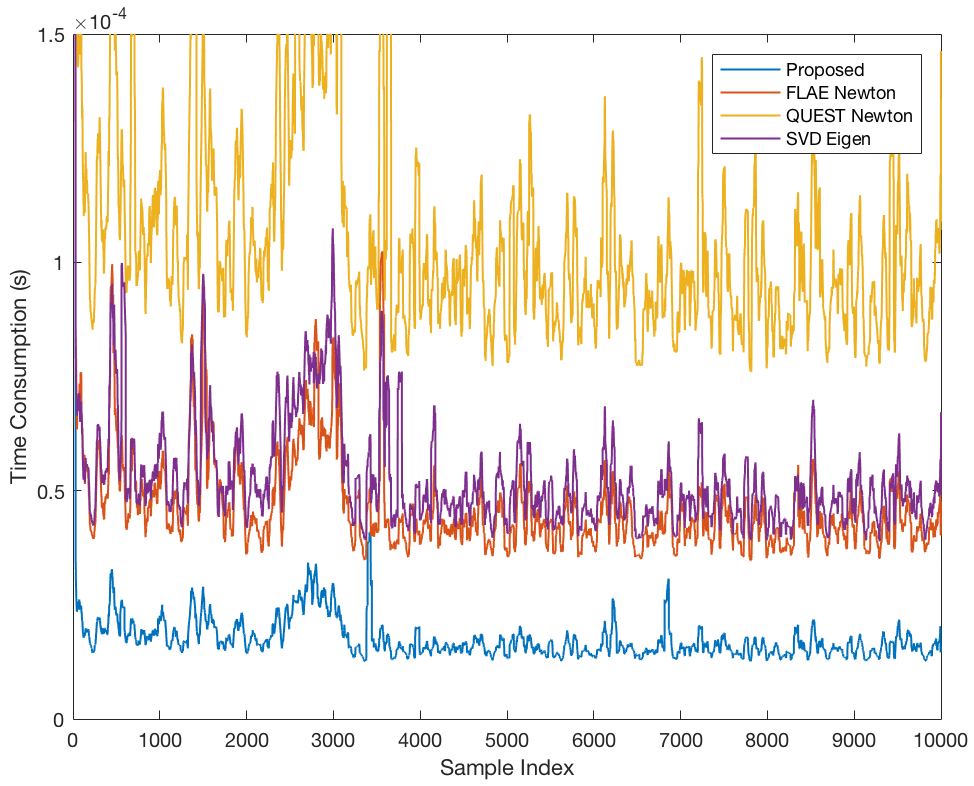
\includegraphics[width=1.0\textwidth]{time.jpg}
% \caption{Execution time consumption of various algorithms.}
% \label{fig:time}
% \end{figure}

\section{Conclusion}
In this paper, we solve the problem of estimating the best rotation for the alignment of two sets of corresponding 3D vectors. It is based on solving the linear equations derived from the formulation of the problem in Geometric Algebra. The method is fast, robust to noise, accurate and simpler than most other methods. Experimental validation of the performance of the proposed algorithm is presented. The results show that the slightly losing accuracy of the proposed method is well worth the huge advance in execution time consumption. For many applications the vector datasets are very huge i.e. the computation time would be more important than slight change of accuracy. Therefore, we hope that the proposed algorithm would be of benefit to such applications.


\section{C++ code}

\begin{lstlisting}[language=C++, caption=C++ code for rotor estimation, basicstyle=\tiny, keywordstyle=\bfseries, label=lst:cppcode, morekeywords={Matrix4d,Vector4d,Vector3d,Quaterniond,sqrt,__m256d,__m128d}]
Quaterniond GAFastRotorEstimatorAVX(
    const vector<Vector3d>& P, 
    const vector<Vector3d>& Q, 
    const vector<double>& w)
{
    Matrix4d H;
    Vector4d R;
    Vector3d S, D;
    double S0, S1, S2, S3, D1, D2, D3, wj;
    const double epsilon = 1e-13;
    const size_t N = P.size(), MAX_STEPS = 12;
    const double* DP = nullptr;
    
    // Compute H = sum_j M_j*M_j
    H.setZero();
    for (register size_t j = 0; j < N; ++j) {
        wj = w[j];
        S = Q[j] + P[j];
        D = P[j] - Q[j];
        S1 = S.x(); S2 = S.y(); S3 = S.z();
        D1 = D.x(); D2 = D.y(); D3 = D.z();
        H(0, 0) += wj*(D1*D1 + D2*D2 + D3*D3); 
        H(1, 0) += wj*(D3*S2 - D2*S3); 
        H(2, 0) += wj*(D1*S3 - D3*S1); 
        H(3, 0) += wj*(D2*S1 - D1*S2);
        H(1, 1) += wj*(D1*D1 + S3*S3 + S2*S2);
        H(2, 1) += wj*(D1*D2 - S2*S1);
        H(3, 1) += wj*(D1*D3 - S3*S1);
        H(2, 2) += wj*(D2*D2 + S3*S3 + S1*S1);
        H(3, 2) += wj*(D2*D3 - S3*S2);
        H(3, 3) += wj*(D3*D3 + S2*S2 + S1*S1);
    }
    // H is lower triangular, complete it to be symmetric
    H.selfadjointView<Eigen::Lower>().evalTo(H);
    // H = (H + epsilon*I)^-1
    H(0, 0) += epsilon; H(1, 1) += epsilon;
    H(2, 2) += epsilon; H(3, 3) += epsilon;
    H = H.inverse().eval();
    // Compute the dominant eigenvector of H using AVX instructions
    for (register size_t j = 0; j < MAX_STEPS; ++j) {
        // H *= H
        // H /= Tr(H)
        wj = 1.0 / H.trace();
        __m256d C1 = _mm256_setr_pd(H(0, 0), H(1, 0), H(2, 0), H(3, 0));
        __m256d C2 = _mm256_setr_pd(H(1, 0), H(1, 1), H(2, 1), H(3, 1));
        __m256d C3 = _mm256_setr_pd(H(2, 0), H(2, 1), H(2, 2), H(3, 2));
        __m256d C4 = _mm256_setr_pd(H(3, 0), H(3, 1), H(3, 2), H(3, 3));
        __m256d weights = _mm256_setr_pd(wj, wj, wj, wj);
        // Perform 4 dot products in parallel
        __m256d xy0 = _mm256_mul_pd(C1, C1);
        __m256d xy1 = _mm256_mul_pd(C1, C2);
        __m256d xy2 = _mm256_mul_pd(C1, C3);
        __m256d xy3 = _mm256_mul_pd(C1, C4);
        __m256d temp01 = _mm256_hadd_pd(xy0, xy1);
        __m256d temp23 = _mm256_hadd_pd(xy2, xy3);
        __m256d swapped = _mm256_permute2f128_pd(temp01, temp23, 0x21);
        __m256d blended = _mm256_blend_pd(temp01, temp23, 0b1100);
        __m256d dotproduct = _mm256_mul_pd(
            _mm256_add_pd(swapped, blended), weights);
        DP = (double*)& dotproduct;
        H(0, 0) = DP[0]; H(1, 0) = DP[1]; H(2, 0) = DP[2]; H(3, 0) = DP[3];
        // Perform 4 dot products in parallel
        xy0 = _mm256_mul_pd(C2, C2);
        xy1 = _mm256_mul_pd(C2, C3);
        xy2 = _mm256_mul_pd(C2, C4);
        xy3 = _mm256_mul_pd(C3, C3);
        temp01 = _mm256_hadd_pd(xy0, xy1);
        temp23 = _mm256_hadd_pd(xy2, xy3);
        swapped = _mm256_permute2f128_pd(temp01, temp23, 0x21);
        blended = _mm256_blend_pd(temp01, temp23, 0b1100);
        dotproduct = _mm256_mul_pd(
            _mm256_add_pd(swapped, blended), weights);
        DP = (double*)& dotproduct;
        H(1, 1) = DP[0]; H(2, 1) = DP[1]; H(3, 1) = DP[2]; H(2, 2) = DP[3];
        // Perform 2 dot products in parallel
        xy0 = _mm256_mul_pd(C3, C4);
        xy1 = _mm256_mul_pd(C4, C4);
        temp01 = _mm256_mul_pd(_mm256_hadd_pd(xy0, xy1), weights);
        __m128d hi128 = _mm256_extractf128_pd(temp01, 1);
        __m128d dotproduct2 = _mm_add_pd(
            _mm256_castpd256_pd128(temp01), hi128);
        DP = (double*)& dotproduct2;
        H(3, 2) = DP[0]; H(3, 3) = DP[1];
    }
    // H is lower triangular, complete it to be symmetric
    H.selfadjointView<Eigen::Lower>().evalTo(H);
    // Choose the column with higher L1 norm
    S0 = H.col(0).lpNorm<1>();
    S1 = H.col(1).lpNorm<1>();
    S2 = H.col(2).lpNorm<1>();
    S3 = H.col(3).lpNorm<1>();
    wj = std::max(S3, std::max(S2, std::max(S0, S1)));
    if (wj == S0) R = H.col(0);
    else if (wj == S1) R = H.col(1);
    else if (wj == S2) R = H.col(2);
    else R = H.col(3);
    R.normalize();
    return Quaterniond(R(0), R(1), R(2), R(3));
}
\end{lstlisting}

\bibliographystyle{abbrv}
\bibliography{rotorestimation}

% ------------------------------------------------------------------------
\end{document}
% ------------------------------------------------------------------------
